\documentclass{article}
\usepackage{enumitem}
\usepackage{amsmath,amssymb,graphicx}
\usepackage{cite}
%\usepackage{Sweave}
\usepackage{tikz}
\usepackage[english]{babel}
\usepackage{url}
\usetikzlibrary{positioning,shapes.geometric,decorations.text}
\begin{document}
%\Sconcordance{concordance:Project-Proposal.tex:Project-Proposal.Rnw:%
1 2 1 1 0 64 1}


\newcommand{\E}{\mathbb{E}}
\newcommand{\indp}{\ensuremath{\perp\hspace{-5pt}\perp}}
\newcommand{\M}{\mathcal{M}}
\newcommand{\given}{\; \mid \;}



\title{\textbf{The Effect of Dieting on Sleep}}
\author{Alex Luedtke, Lucia Petito, and Steven Pollack}
\date{}
\maketitle

\section{Specify the Question}

Recently researchers have tried to relate successful dieting to sleeping habits.  A relationship between obesity and sleep cycles has been established: both oversleeping and sleep deprivation are associated with an increased Body Mass Index (BMI) [REFERENCE]. 

Nonetheless, little work has been done to consider the opposite relationship. Specifically, we are interested in parsing the causal effect of attempting to lose weight on a person's sleep habits (average hours of sleep/night). While the health benefits associated with losing weight are well documented, it is not currently known if dieting has a negative, positive, or no effect on an individual's sleep habits.

There are reasonable explanations for all possible outcomes of this analysis.  An increased interest in one's diet could indicate an increased interest in one's overall health.  Because doctors advise their patients to consistently get enough sleep each night to maintain a healthy lifestyle, it would be reasonable to see more hours of sleep in people who are dieting.  On the other hand, dieting has profound psychological and hormonal effects, which could cause a disruption to normal sleep patterns and result in less sleep on average [REFERENCE].

For the purposes of this analysis, our population of interest is adults ages 25-79 who are not pregnant, have never been diagnosed by a doctor with a sleep disorder, and live in the United States.  We used the National Health and Nutrition Examination Survey (NHANES) data from 2009-2010 \cite{data} from the following questionnaires: ``Demographic Variables and Sample Weights," ``Weight History 16 Years and Older," and ``Sleep Disorders" \cite{questionnaire}.

NHANES is a multi-stage survey of the U.S. population that the Center for Disease Control and Prevention (CDC) conducts every 2 years.  They sample counties first, then ``segments'' (which can be as small as street blocks to as big as neighborhoods: determined by population density), then households, and finally individuals.  It aims to study a wide range of topics such as cardiovascular disease, obesity, physical fitness and physical functioning, reproductive history and sexual behavior, etc.  Each individual participates in an interview and a physical examination.  The sample is chosen to represent the U.S. population of all ages.  To produce reliable statistics, NHANES over-samples persons 60 and older, adolescents, African Americans, and Hispanics among others [REFERENCE if not in other cited nhanes documents].  

However, to protect the privacy of the participants, the CDC strips the data of any information that would allow an analyst to find an individual.  This process mostly removes geographic identifiers; in particular, they remove all information about the first three stages of their multistage sampling procedure.  Unfortunately, this removal of information means that we cannot fully replicate their sampling methodology.

Our baseline covariates are:
\vspace{0.5cm}

\begin{table}
\caption{Table: Baseline Covariates}
\begin{tabular}{| p{3cm} | p{7cm} |}
\hline
When the interview was conducted & 1 for November 1, 2009 - April 30, 2010, 2 for May 1, 2009 - October 31, 2010\\
\hline
Subject Gender & 1 for Male, 2 for Female\\
\hline
Age in Months & 300-959, or 25-79 years\\
\hline
Race/Ethnicity & 1 for Mexican American, 2 for Other Hispanic, 3 for Non-Hispanic White, 4 for Non-Hispanic Black, 5 for Other Race\\
\hline
Education Level & 1: less than 9th grade, 2: 9-11th grade (including 12th grade with no diploma), 3: high school grad/GED or equivalent, 4: some college or AA degree, 5: college graduate or above\\
\hline
Marital Status & 1: married, 2: widowed, 3: divorced, 4: separated, 5: never married, 6: living with partner\\
\hline
Annual Household Income & 14 levels, \$0-\$24,999 by \$5,000, \$25,000-\$74,999 by \$10,000,  \$75,000 - \$99,999, \$100,000 and over, \$20,000, \$20,000\\
\hline
Body Mass Index & continuous values from ~15-50 [Note: this is a combination of subject weight and subject height, computed according to the formula used by the CDC \cite{bmi}\\
\hline
\end{tabular}
\end{table}


\vspace{0.5cm}
%\caption{These covariates were collected in an interview conducted by researchers at the CDC.}

This data set contains many individuals that have missing data.  The percentage missing in each covariate is in Table \ref{}[REFER TO TABLE].  We implemented a complete-case analysis instead of implementing an imputation procedure for this study. Specifically, we deleted all people who responded ``refused" or ``don't know" or are missing data for Annual Household Income, Marital Status, Education Level, and Interview Time Period.  We deleted all people who were younger than 25 and older than 79, all pregnant women, and all people who had ever been diagnosed by a doctor with a sleep disorder (or who responded that they ``don't know").  

We also coarsened the categories for several of the variables.  We were interested in the ``Marital Status'' variable because it described whether or not the individual had a stable relationship in their life, so we collapsed it into ``married or living with partner'' vs ``else.''  Because a significant number of people replied ``\$20,000'' and ``\$20,000'' to the annual household income question, we decided to define all individuals as such, including those for which we had more detailed information.  We also collapsed the bottom two categories for ``Education Level'' into one category: ``less than 11th grade.''

[INSERT TABLE]

% \section{Potential Sources of Bias}
% 
% We would have liked to exclude all people who are on medications that cause excessive weight gain as a side effect, such as anxiety and depression medications.  Unfortunately, our data set does not include this covariate.  
% 
% Our annual household income data 

\section{Specify the Causal Model}

Our observational data structure is $O=(W,A,Y) \sim P_0$. Our endogenous variables are $W$, $A$, and $Y$, where $W$ is as listed in Table 1.

\begin{itemize}
\item When the interview was conducted (1: November 1, 2009 - April 30, 2010, 2: May 1, 2009 - October 31, 2010)
\item Subject Gender (1: Male, 2: Female)
\item Age in Months (300-959, or 25-79 years)
\item Race/Ethnicity (1: Mexican American, 2: Other Hispanic, 3: Non-Hispanic White, 4: Non-Hispanic Black, 5: Other Race)
\item Education Level (1: less than 11th grade (including 12th grade with no diploma), 3: high school grad/GED or equivalent, 4: some college or AA degree, 5: college graduate or above)
\item Marital Status (1: married or living with partner, 0: else)
\item Annual Household Income (0: \$20,000, 1: \$20,000)
\item Body Mass Index (continuous values from ~15-50) [Note: this is a combination of subject weight and subject height, computed according to the formula in [REFERENCE]]
\end{itemize}

$A$ is the individual's response to the survey question: ``During the past 12 months, have you tried to lose weight?", and $Y$ is the individual's response to ``How much sleep do you usually get at night on weekdays or workdays?''  

Our exogenous variables are $U = (U_W, U_A, U_Y) \sim P_U$. We make no assumption on the joint distribution of $U$.  

We make no exclusion restrictions on our data and no assumptions on the functional forms of $W$, $A$, or $Y$.

Because the data for $W$, $A$, and $Y$ was gathered simulateneously, temporal assumptions are needed to specify a causal model. We assume that all variables in $W$ occur temporally before the variables in $A$ and $Y$, and that $A$ occurs before $Y$. We first discuss temporal ordering between $W$ and $A$. First, note that the claim that the subjects gender, age, race, and BMI one year ago appear temporally before their decision to diet in the last twelve months is clearly true. When the interview was conducted also clearly occurs before the answer to the question in $A$, and thus we have temporal ordering here as well. Nonetheless, we do not necessarily temporal ordering for education level, marital status, and annual household income. All of the same observations hold for temporality between $W$ and $Y$.

Temporal assumptions between $A$ and $Y$ are somewhat justifiable due to the wording of the question in $A$, specifically because the question specifically asks whether the individual has tried to lose weight in the last year. The variable $Y$, on the other hand, asks about average sleep habits, which we believe indicates a response to a more recent phenomenon than the last year. Nonetheless, violations of this temporality may occur if the individual started to try to lose weight recently or if the individual considers long-term (more than a month) sleep habits when answering the question in $Y$. Though our temporality between $A$ and $Y$ is by no means perfect, we believe this tempol ordering is far more likely than the reverse, namely $Y\rightarrow A$. 

We now proceed as though our temporal assumptions are true, yielding the SCM:

\begin{align*}
W &= f_{W}(U_{W}) \\
A &= f_{A}(W,U_{A}) \\
Y &= f_{Y}(W,A,U_{Y}) \\
\end{align*}

\begin{figure}[h]
    \centering
    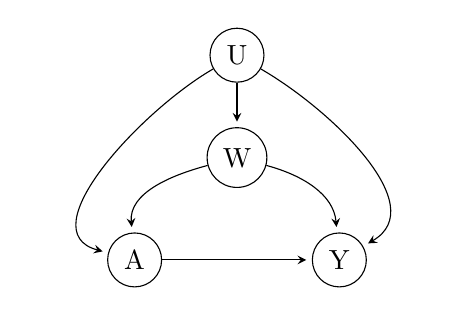
\begin{tikzpicture}[->, shorten >=2pt, >=stealth, node distance=1cm,
                        pil/.style={->,thick,shorten =2pt,},scale=0.65
                        ]
    \node[circle,draw] at (4,2) (1) {W};
    \node[circle,draw] at (2,0) (2) {A};
    \node[circle,draw] at (6,0) (3) {Y};
    \node[circle,draw] at (4,4) (4) {U};
    \draw[->] (1) to [out=195,in=95] (2);
    \draw[->] (2.east) -- (3.west);
    \draw[->] (1) to [out=345,in=95] (3);
    \draw[->] (4.south) -- (1.north);
    \draw[->] (4) to [out=210,in=165] (2);
    \draw[->] (4) to [out=330,in=30] (3);
    \end{tikzpicture}
  \caption{Simplified DAG -- no independence assumptions on $U$'s.}
  \label{fig:DAG}
\end{figure}


\section{Specify the Causal Parameter of Interest}

Since the intervention is a point treatment, our counterfactual is $Y_{a}$: the average sleep an individual would get, if they, possibly contrary to fact, had (or had not) attempted to lose weight.

We are interested in measuring the average treatment effect (ATE) of attempted weight loss on average sleep:

$$\Psi(P_{U,X}) = \E_{U,X}[Y_1] - \E_{U,X}[Y_0]$$

\section{Assess Identifiability and Positivity}
\label{sec:assumptions}

Since $\Psi$ is the ATE, we need to satisfy backdoor criterion to identify G-computation with $\Psi$:
   $$Y_{a} \indp A \mid W$$

For identfiability, we need $U_{A} \indp U_{Y}$. That is, we need there to be no unmeasured common causes between attempting to lose weight and average number of hours of sleep per weekday night. We also need either
    \begin{itemize}
      \item $U_{A} \indp U_{W}$: No unmeasured common causes between an individual's attempt to lose weight and their baseline covariates. This assumption is somewhat plausible given the number of baseline covariates measured, but may not hold.
      \item $U_{W} \indp U_{Y}$: No unmeasured common causes between average hours of sleep per weekday night and baseline covariates. This assumption seems less plausible. For instance, an individual's stress level one year ago likely has a causal effect on their current relationship status and household income. This variable also likely has a causal relationship with current stress, which in turn may modify sleep habits.
    \end{itemize}

\begin{center}
    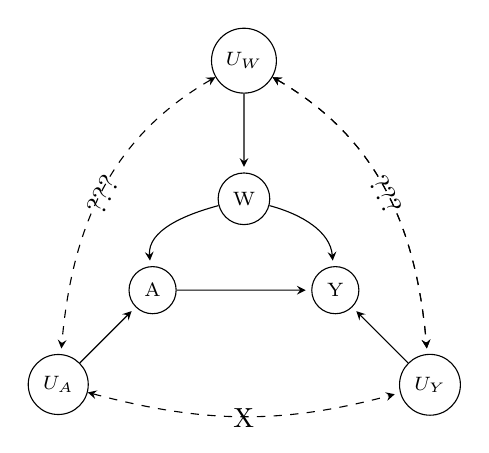
\begin{tikzpicture}[->, shorten >=2pt, >=stealth, node distance=1cm,
                        pil/.style={->,thick,shorten =2pt,},scale=0.65,font=\scriptsize
                        ]
    \node (A) [circle,draw] {A};
    \node (W) [circle,draw,above right=of A] {W};
    \node (Y) [circle,draw,below right=of W] {Y};
    \node (UA) [circle,draw,below left=of A] {$U_A$};
    \node (UW) [circle,draw,above=of W] {$U_W$};
    \node (UY) [circle,draw,below right=of Y] {$U_Y$};
    \draw[->] (W) to [out=195,in=95] (A);
    \draw[->] (A.east) -- (Y.west);
    \draw[->] (W) to [out=345,in=95] (Y);
    \draw[->] (UW.south) -- (W.north);
    \draw[->] (UA) to [out=45,in=225] (A);
    \draw[->] (UY) to [out=135,in=315] (Y);
    \draw[dashed,<->] (UW) to [out=330,in=95] (UY);
    %\pgftransformyshift{-.65cm}
    %\draw[decoration={text along path, text={X},text align={center}},decorate] (UA) to
                      [out=345,in=195] (UY);
    \draw[dashed,<->,postaction={decorate,decoration={raise=-4pt,text along path,text align=center,text={X}}}] (UA) to [out=345,in=195] (UY);
    \draw[dashed,<->,postaction={decorate,decoration={raise=-4pt,reverse path,text along path,text align=center,text={???}}}] (UW) to [out=210,in=85] (UA);
    \draw[dashed,<->,
    postaction={decorate,
    decoration={raise=-4pt,text along path,text align=center,text={???}}}] (UW) to [out=330,in=95] (UY);
    \end{tikzpicture}
\end{center}

We must also address the issue of positivity.  We do not believe that trying to lose weight or not trying to lose weight occurs with probability $0$ given any set of covariates $W$.  Thus we believe our theoretical positivity requirements are met.  However, practical positivity violations are very prevalent given that $W$ is high dimensional.  If we only consider those variables in $W$ that are categorical (Gender, Race/Ethnicity, Education Level, Marital Status), we only have two strata where no people tried to lose weight:

\begin{tabular}{| l | l | l | l |}
\hline
 Gender & Race & Education & Marital Status \\
\hline
Male & Other & Less than HS & Unmarried/not living with partner \\
Female & Other & HS & Married/living with partner \\
\hline
\end{tabular}

\section{Commit to a Statistical Model and Target Parameter of the Observed Data Distribution}

We still have no assumptions on the functional forms of $f_W, f_A$, and $f_Y$, so we choose the non-parametric model $\mathcal{M}$ of distributions compatible with our SCM.  

We are still interested in the ATE, so our target parameter of the observed data distribution (assuming that we have a simple random sample of 4,077 individuals) is

$$\psi_0 = \sum_{w}\Big[\E_0(Y|A=1,W=w)-E_0(Y|A=0,W=w)\Big]P_0(W=w)$$

\section{Estimate the Chosen Parameter of the Observed Data Distribution}

We proceed with estimation even if cannot fully accept $U_A \indp U_W$ or $U_W \indp U_Y$ as presented in Section \ref{sec:assumptions}. If the assumptions hold, then we know that our estimates are directly estimating a causal parameter. Otherwise, we consider the estimates valuable pieces of information, albeit with known shortcomings. We will estimate the ATE in the following ways: 

\begin{itemize}
  \item Simple Substitution:
    \[
      \psi_0 \approx \frac{1}{n}\sum_{i=1}^{n}\Big(\bar{Q}_{n}^{0}(1,W_i) - \bar{Q}_{n}^{0}(0,W_i)\Big)
    \]
Where $\bar{Q}_{n}^{0}(a,W_i)$ is an estimate of $\E_0(Y|A=a,W)$.
  \item IPTW:
  \[
    \psi_{0} \approx \frac{1}{n}\sum_{i=1}^{n} \left(\frac{I(A_i=1)}{\hat{g}_n(A_i \mid W_i)} - \frac{I(A_i=0)}{\hat{g}_n(A_i \mid W_i)} \right)Y_i
  \]
Where $\hat{g}_n(a_i \mid W_i)$ is an estimate of $P_0(A=a_i|W_i)$.
  \item TMLE:
  \[
    \psi_{0} \approx \frac{1}{n}\sum_{i=1}^{n}\left( \bar{Q}_{n}^{1}(1,W_i) - \bar{Q}_{n}^{1}(0,W_i)\right)
  \]
Where $\bar{Q}_{n}^{1}(a,W_i)$ is a targed estimate of $\E_0(Y|A=a,W)$ \cite{tmle}.
\end{itemize}

We obtain our estimates of $\hat{g}$ and $\bar{Q}_n^0$ using the candidate library in SuperLearner shown in Table \ref{tab:sl.lib} \cite{superlearner}.
\begin{table}[ht!]
\begin{tabular}{l | l}
Default Algorithms & Custom GLM's \\
\hline
SL.mean & $Y \sim A$ \\
SL.earth & $Y \sim A \times Gender \times RaceEth + MarStat \times HHInc$ \\
SL.rpartPrune & $+ AgeMonths$:$Gender + EduLevel + AgeMonths $ \\
SL.ridge & $Y \sim A \times Gender \times MarStat$ \\
SL.glmnet &  $Y \sim A \times Gender \times AgeMonths \times HHInc$ \\
\end{tabular}
\caption{SuperLearner library. Note that the library includes both simple functions such as SL.mean and the custom $Y\sim A$ and higher level functions such as SL.earth (similar to SL.polymars) and SL.rpartPrune.}
\label{tab:sl.lib}
\end{table}

\section{Interpret Results}



\bibliography{mybib}{}
\bibliographystyle{plain}


\end{document}
